\section{Affine and cyclic menus with pairwise correlation certificates}
\label{sec:menus}

\subsection{Operation supports and exact selection}
For an unordered pair $e=\{g,h\}$ put $g_e=h_{gh}+h_{hg}$.
A plan partitions the ordered group labels into three nonempty blocks.
Within each block, recursively split its ordered list after
$\floor{k/2}$ elements and merge the two boundary tables. Finally contract
the three block tables. This gives $r-3$ binary merges and one final
triangle, hence $r-2$ operations.

Multiplying each of the three linear forms in \eqref{eq:matrix} by five
gives a support mask $v\in\{0,2,5\}^{\binom r2}$. Its value is zero
inside a class of the operation's tripartition, two on the discounted
class pair, and five on the other two class pairs. Let $\mathcal V_j$
contain all $3(r-2)$ masks of plan $j$. After singleton caching, plan $j$
has local operation exponent
\[
 F_j(g)=\frac15\max_{v\in\mathcal V_j}v\cdot g.
\]
All matrix operations, not only the last triangle, are included.

\begin{theorem}[Pairwise correlation certificate]\label{thm:gram}
For $q$ fixed plans on $r$ groups, let $D_{ij}$ be any explicit upper bound
on $v\cdot w$ for $v\in\mathcal V_i,w\in\mathcal V_j$, and put
$S=\sum_{i,j}D_{ij}$. Selecting the least-cost plan gives local time and
storage at most
\[
 \poly(s)2^{(b_r+o(1))\K(M,u)},\qquad
 b_r^2=\frac{2S}{25q^2r^2}.
\]
The selector is exact and polynomial time in the original size parameter.
\end{theorem}
\begin{proof}
For the given nonnegative $g$, choose a maximizing $v_i$ from each menu.
Then
\[
 \min_i F_i(g)\le\frac1{5q}\left(\sum_i v_i\right)\cdot g,
 \qquad
 \left\|\sum_i v_i\right\|_2^2
       =\sum_{i,j}v_i\cdot v_j\le S.
\]
Give both directed orientations of edge $e$ the weight
$(\sum_i v_i)_e/(5q)$. Its squared norm is at most $2S/(25q^2)$.
Lemma~\ref{lem:entropy} proves the time estimate. The possible choices of
supports form a fixed finite set, so the error remains uniform although
the selected plan depends on the input. No minimax equality is assumed.

For selection, compute the exact positive integers
\[
 P_i=\max_{v\in\mathcal V_i}
       \prod_{\{g,h\}}
       (|\mathcal I_{gh}|\,|\mathcal I_{hg}|)^{v_{\{g,h\}}}
\]
and choose the smallest. Comparing them is equivalent to comparing
$F_i(g)$; no approximate logarithm is needed. Their bit lengths are
polynomial and $q,r$ are fixed. Finally every table is an input or output
of a selected operation, whose exponent dominates its size by
\eqref{eq:matrix}. A fixed number of tables introduces only a constant
factor. The time to evaluate the singleton entries is charged separately.
\end{proof}

The earlier support-tuple method has an exponential dependence on the
number of plans, even though this remains a constant asymptotically. The
new certificate requires $q^2$ pair comparisons. It bounds the simultaneous
sum of supports rather than asserting that all pairwise maxima can occur
at once. Such an assertion would be unnecessary and generally false.

\subsection{Four parallel classes on nine points}
Label the groups by $x\mapsto(x\bmod3,\floor{x/3})\in\mathbb F_3^2$.
For each of the four functionals
\[
 (a,b)\in\{(1,0),(0,1),(1,1),(1,2)\},
\]
use its three
level sets as the final blocks. Within each level set use increasing
integer order. These four plans are
\[
\begin{split}
 &(0,3,6)\mid(1,4,7)\mid(2,5,8),\\
 &(0,1,2)\mid(3,4,5)\mid(6,7,8),\\
 &(0,5,7)\mid(1,3,8)\mid(2,4,6),\\
 &(0,4,8)\mid(1,5,6)\mid(2,3,7).
\end{split}
\]
\begin{figure}[ht]
\centering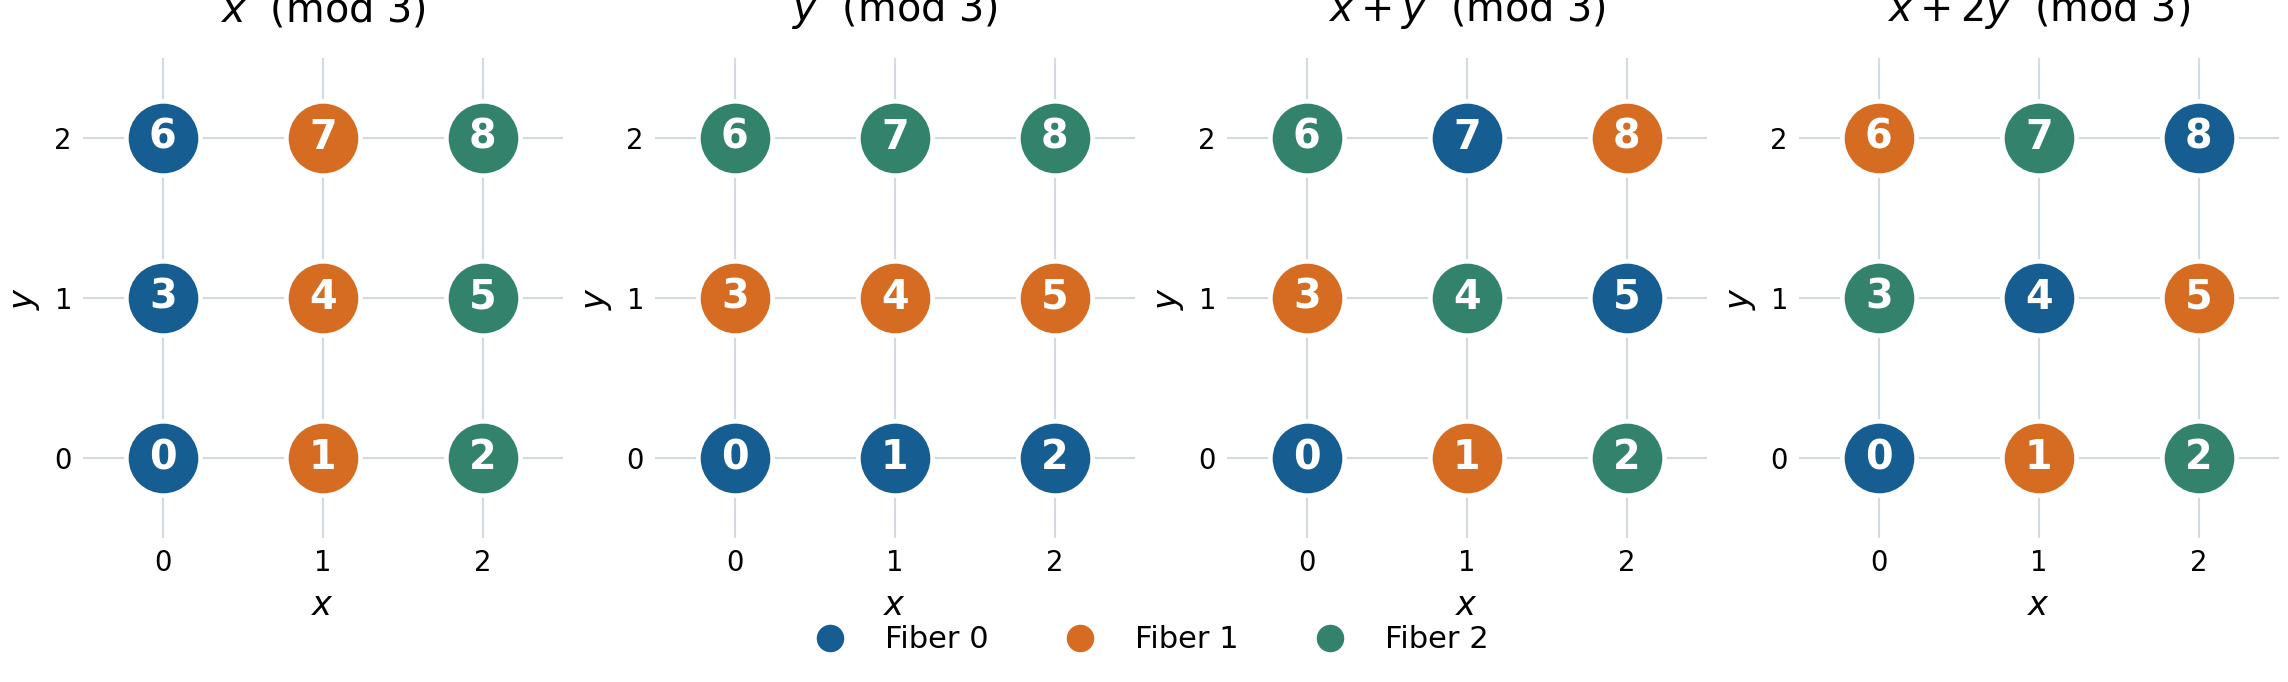
\includegraphics[width=\textwidth]{figures/affine_classes.png}
\caption{The four parallel classes of $\mathbb F_3^2$. In each panel,
colors denote the three fibers of the indicated linear functional, with
arithmetic modulo three. Labels are the group numbers. Each fiber is one
final block; straight Euclidean lines are not required to display the
modular wraparound.}
\end{figure}

Each plan has 21 masks. Exact pairwise maxima are
\[
 D_{ii}=486,\qquad D_{ij}=288\quad(i\ne j).
\]
Thus $S=4\cdot486+12\cdot288=5400$ and
\begin{equation}\label{eq:b9}
 b_9^2=\frac13.
\end{equation}
This can be checked by 7,056 mask-pair dot products, not by sampling
entropy vectors. The independent implementation represents each support
as $v=5\mathbf1_C-3\mathbf1_D$ and uses
\begin{equation}\label{eq:intersection}
 v\cdot w=25|C\cap C'|-15(|D\cap C'|+|C\cap D'|)+9|D\cap D'|.
\end{equation}

There is also a geometric explanation for the largest off-diagonal value.
Two distinct directions have a one-point intersection between every pair
of their lines. For the final triangles, the two crossing edge sets have
intersection size 18; either discounted set meets the other crossing set
in 6 edges, and the discounted sets meet in 2. Equation~\eqref{eq:intersection}
then gives $25\cdot18-15(6+6)+9\cdot2=288$.
For completeness, the exact off-diagonal bounds by operation type are
\[
\begin{array}{c|rrr}
 & (1,1,7)&(1,2,6)&(3,3,3)\\\hline
 (1,1,7)&204&208&215\\
 (1,2,6)&208&240&260\\
 (3,3,3)&215&260&288
\end{array}
\]
where the triples specify the class sizes of an operation. The finite
enumeration covers all of them, including the ordering-dependent internal
merges.

\subsection{Thirteen cyclic plans}
Take the ordered seed
\[
 (11,2,8,9,7)\mid(10,1,0,5)\mid(6,4,3,12)
\]
and add $d$ modulo 13 to every label for $0\le d<13$. The within-block
orders remain the shifted orders; sorting them would define different
plans. There are 33 masks per plan. The maximum-dot matrix is circulant,
with first row
\[
 (1064,647,651,713,647,709,651,651,709,647,713,651,647).
\]
Its row sum is 9,100. Hence $S=118,300$ and
\begin{equation}\label{eq:b13}
 b_{13}^2=\frac{56}{169}.
\end{equation}
The checker exhausts 184,041 mask-pair dot products. The seed was found by
an exploratory search. Its validity depends only on this explicit seed
and the complete integer checks; no optimality or exhaustive seed search
is claimed.

For the final six-group tail use
$(0,1)\mid(2,3)\mid(4,5)$. Its final triangle has maximum squared mask
norm 216 and each internal merge at most 204, giving
$b_6^2=2\cdot216/(25\cdot6^2)=12/25$.

\subsection{Why the gain is not merely schedule slack}
The earlier best three-plan nine-group certificate has
$b_{9,\rm old}^2=6608/18225$ \cite{treecert}. In the same packing model,
the root taper fraction satisfies $\eta_0<1/(20\log_2 9)$. Even pushing
that certificate to its boundary leaves root coefficient at least its
infimum
\[
 \kappa b_{9,\rm old}\sqrt{20\log_2 9}
 =30.731244617454\ldots,
\]
which is larger than our complete time coefficient. Thus our improvement
cannot be reproduced solely by reclaiming the rational slack of that
particular old root certificate. This is a statement about the displayed
certificate model; it is not an algorithmic lower bound or a global
optimization over all methods in the corpus.
